\documentclass[a4paper,11pt]{article}
\usepackage[T1]{fontenc}
\usepackage[utf8]{inputenc}
\usepackage{xcolor}
\usepackage{geometry}
\usepackage{subfig}
\geometry{left=2.5cm,right=2.5cm,top=2.5cm,bottom=2.5cm}
\usepackage{multicol}
\usepackage{fancyhdr}
\linespread{1.5}
\colorlet{shadecolor}{gray!40}
\usepackage{listings}
\usepackage{subcaption}
\usepackage{pdfpages}
\lstdefinestyle{mystyle}{
	%backgroundcolor=\color{shadecolor}
	commentstyle=\footnotesize\color{blue},
	keywordstyle=\color{red},
	numberstyle=\footnotesize\color{black},
	stringstyle=\color{black},
	basicstyle=\footnotesize,
	breakatwhitespace=false,
	breaklines=true, captionpos=b,
	keepspaces=true, numbers=left,
	numbersep=5pt, showspaces=false,
	showstringspaces=false, showtabs=false,
	tabsize=2,	
}
\lstset{style=mystyle}
\setlength{\parindent}{1.25cm}


\usepackage{amsmath}
\usepackage{graphicx}
\usepackage{hyperref}
\usepackage{fancyhdr}
\usepackage{tocloft}

\begin{document}

	\section{Opis programu transformaty Hopf Cole'a}
Program komputerowy został napisany na podstawie wzorów~\ref{14a}:
\begin{equation}
\label{14a}
\begin{split}
    \theta_{i,j+1}=(1-2r)\theta_{i,j}+2r\theta_{i+1,j}, \ \ i=0\\
    \theta_{i,j+1}=2r\theta_{i-1,j}+(1-2r)\theta_{i,j}+r\theta_{i+1,j}, \ \ 1\le i\le N-1\\
    \theta_{i,j+1}=2r\theta_{i-1,j}+(1-2r)\theta_{i,j}
\end{split}
\end{equation}.
Natomiast równanie na u zostało zrobione z wzoru:
\begin{equation}
    u(x_i,t_j)=-\frac{\beta}{h}\left(\frac{\theta_{i+1,j}-\theta_{i-1,j}}{\theta_{i,j}}\right)\ \ 1\le i\le N-1
\end{equation}.
Gdzie $\beta$ jest współczynnikiem lepkości, h krokiem przestrzennym, a k - krokiem czasowym.
	\subsection{transformataHopfCole.h}
	Plik nagłówkowy zawiera definicje metod klasy transformaty. Na początku zostały dołączone wszystkie klasy, które są potrzebne do działania programu, jak pokazuje listing~\ref{poczatekPlikuH}.
		\begin{lstlisting}[caption={początek pliku transformataHopfCole.h},label={poczatekPlikuH}, language=C++]]
		#pragma once
		#include <vector>
		#include <cmath>
		#include <algorithm>
		#include <conio.h>
		#include <math.h>;\end{lstlisting}
	Następnie zostały napisana dyrektywa, która pozwala na używanie wszystkich nazw z~przestrzeni nazw "std" bez konieczności ich niefiksowania. Przestrzeń nazw definiuję standardowych klas i~funkcji z~biblioteki standardowej w~C++, takich jak "cout", "vecotr", "string", co skraca trochę kod. Potem zostały definiowanie stała Pi oraz~e, jeśli nie są szybciej zdefiniowanie, co przedstawia listing~\ref{definiowanieStałych}. 
	\begin{lstlisting}[caption={początek pliku definiowanieStałych},label={zdefiniowanie stałych}, language=C++]]
		using namespace std;
		#ifndef M_PI
		#define M_PI 3.14159265358979323846
		#endif
		
		#ifndef M_E
		#define M_E 2.71828182845904523536
		#endif\end{lstlisting}
		
	Potem została zdefiniowania klasa, w~której są wszystkie metody oraz stale potrzebnie do pracy programu.
			\begin{lstlisting}[caption={klasa tranformataHopfCofe},label={klasa}, language=C++]
			class transformataHopfCole {
				const double k = 0.005, h = 0.1;
                const int N = 1 / h + 1;      // liczba punktów siatki
				const double n = ((0.5 * pow(h, 2)) / k) - 0.01;
				const double r = n*k / pow(h, 2);
				double t = 0;
				
				vector<double>theta;
				vector<double>mu;
				vector<double> inicjacja_u(); //wzror 4 z pracy
				vector<double>inicjacjaThetaX0(); //wzor 8 z pracy
				vector<double>liczenieThetaOdCzasu();
				
				vector<double>liczenieMu(vector<double>newMu);//wzor 15
				void zapisDoPliku(vector<double> Theta, double newT);
				public:
				void wynikiKonczowe();
			};\end{lstlisting}
		Pierwsza stała oznacza liczbę punktów, "k" odpowiada za krok czasowy, natomiast "h" za krok przestrzennego w~dyskretyzacji przestrzennej.\\
		W~8~i~9~linii zostały inicjowanie vectoru, gdzie zostaniom zapisanie wyniki programu. W~kolejnych trzech linach zostały już zdefiniowanie klasy, które krok po kroku będą obliczały wynik końcowy oraz w linii~14.\\
		Przedostatnia prywatna metoda służy, by otrzymanie wyniki zostały zapisanie do pliku. Ostaną metodą jest "wynikiKoncowe()", która jest publiczna. 
		\subsection{transformataHopfCole.cpp}
		W kolejnym pliku znajdują się ciała metod klasy. Na początku pliku zostały załączone biblioteki oraz własna klasa do prawidłowego działania programu. 
					\begin{lstlisting}[caption={poczadek pliku transformataHopfCole.cpp},label={poczadek.cpp}, language=C++]
#include "transformataHopfCole.h"
#include <iostream>
#include <fstream>
#include <string>\end{lstlisting}
	\	Następne jest ciało metody inicjacjaThetaX0 co przedstawia listing~\ref{inicjacjaThetaX0}. Ta metoda ma na celu inicjacji~$\theta$ dla czasu zerowego. Pętla służy do wygenerowana dla wszystkich~$\theta$ wartości początkowych, z~których potem zostaną wykorzystanie do dalszych obliczeń. Pod koniec metody zostanie wywołania kolejna metoda, która zapiszę wartości do pliku tekstowego oraz zwrócenie tych wartości do vectora.
						\begin{lstlisting}[caption={ciało metody inicjacjaThetaX0},label={inicjacjaThetaX0}, language=C++]
		vector<double> transformataHopfCole::inicjacjaThetaX0() {
			vector<double>newTheta;
			for (int i = 0; i < N; ++i) {
				double potega = (-1 / (2 * M_PI * n)) * (1 - cos(M_PI * (i * h)));
				newTheta.push_back(exp(potega));
			}
			zapisDoPliku(liczenieMu(newTheta), 0);
			return newTheta;
			}\end{lstlisting}
		Kolejną metodą jest "liczenieThetaOdCzasu" (listing~\ref{liczenieThetaOdCzasu}). Metoda ma na celu policzenie~$\theta$ dla czasu. Pierwsza pętla służy do policzenie~"t", czyli kroku czasowego. Potem jest zdefiniowany nowy vector, w którym zostaną zapisanie nowe wartości. Druga pętla służy do policzenia dla $\theta$ od~1 do~N-1. Po drugiej pętli zostaną nadpisanie wartości dla theyaDlaCzasu nowymi wartościami dla konkretnego czasu. Na końcu jest wywołania metoda, która otrzymanie wyniki zapiszę do pliku. Na samym końcu zostanie zwrócony vector.   
								\begin{lstlisting}[caption={ciało metody liczenieThetaOdCzasu},label={liczenieThetaOdCzasu}, language=C++]
vector<double> transformataHopfCole::liczenieThetaOdCzasu() {
	vector<double>thetaDlaCzasu(N);
	thetaDlaCzasu = theta;
	for (int j = 1; j < 3000; ++j) {
		t = j * k;
		vector<double>v(N);
		v[0] = (1 - 2 * r) * thetaDlaCzasu[0] + 2 * r * thetaDlaCzasu[1]; //warunki brzegowe  
		v[N - 1] = 2 * r * thetaDlaCzasu[N - 2] + (1 - 2 * r) * thetaDlaCzasu[N - 1];
		for (int i = 1; i < (N - 1); ++i) {
			double wynik = r * thetaDlaCzasu[i - 1] + (1 - 2 * r) * thetaDlaCzasu[i] + r * thetaDlaCzasu[i + 1];
			v[i] = wynik;
		}
		thetaDlaCzasu = v;
		zapisDoPliku(liczenieMu(thetaDlaCzasu), t);
		
	}
	return thetaDlaCzasu;
	}\end{lstlisting}
Kolejną metodą jest "liczenieMu", która wykorzystuję $\theta$ od czasu do policzenia $u(x,t)$. Na wyraz 0 i~(N-1) jest przypisana wartość~0, co wynika z warunki początkowego i~końcowego. Kolejne wartości są liczone w pętli for, jak pokazuje listing~\ref{liczenieMu}. 
\begin{lstlisting}[caption={ciało metody liczenieMu},label={liczenieMu}, language=C++]
vector<double> transformataHopfCole::liczenieMu(vector<double> newMu) {
	vector<double>newMu1(N);
	newMu1[0] = 0;//warunek poczatkowy
	newMu1[N - 1] = 0;//warunek koncowy
	for (int i = 1; i < (N - 1); ++i) {
		newMu1[i] = (-(n / h) * ((newMu[i + 1] - newMu[i - 1]) / newMu[i]));
	}
	
	return newMu1;
	}\end{lstlisting}
Przedostatnią metodą jest "zapisDoPliku", który ma na celu otrzymanych wyników zapisach do pliku. Na początku jest inicjowany string, który będzie nazwą pliku. Potem program tworzy nowy plik, jeśli nie istnieje, jak istnieje to zawartość zostanie zastąpiona. Potem w warunku jest sprawdzenie czy udało się otworzyć plik, jeśli nie to pojawi się odpowiednia informacja. Pętla for ma na celu zapisanie wszystkich punktów do pliku. Na końcu program zamyka plik, gdy już skończył pracę.
\begin{lstlisting}[caption={metoda zapisDoPliku},label={ZapisDoPliku}, language=C++]
void transformataHopfCole::zapisDoPliku(vector<double> newMu, double newT) {
	string nazwaPliku = "Wyniki1DlaT" + to_string(newT) + ".txt";
	std::ofstream plik(nazwaPliku);
	
	// Sprawdzamy, czy plik został otwarty poprawnie
	if (!plik) {
		std::cerr << "Nie można otworzyć pliku!" << std::endl;
		return;
	}
	for (int i = 0; i < size(newMu); ++i) {
		
		plik << (i * h) << " " << newMu[i] << '\n';
	}
	
	// Zamykamy plik
	plik.close();
}\end{lstlisting}
Ostaną metodą są "wynikiKoncowe", który na początku wywołuje metodę "inicjacjaThetaX0", następnie "liczenieThetaOdCzasu". Kolejne metody nie są potrzebne by je wywołać, z powodu, że metoda "liczenieThetaOdCzasu" wywołuje metodę która liczy $u(x,t)$ i metodą, która zapisuję dane do pliku. 
\begin{lstlisting}[caption={metoda wynikiKonczowe},label={wynikiKonczowe}, language=C++]
void transformataHopfCole::wynikiKonczowe() {
	theta = inicjacjaThetaX0();
	theta = liczenieThetaOdCzasu();
	}\end{lstlisting}
\subsection{transformata.cpp}
Kolejnym plikiem jest transformata.cpp, który ma funkcję główną main.cpp. Która na początku ma dołączona klasę. Następnie w main tworzy się obiekt klasy transformataHopfCole, a następnie wywołuję się metodę klasy, by program policzył nam wyniki. 
\begin{lstlisting}[caption={transformata.cpp},label={transformata}, language=C++]
#include "transformataHopfCole.h"
int main()
{
	transformataHopfCole Burger;
	Burger.wynikiKonczowe();
}
\end{lstlisting}
\section{wyniki}
Wygenerowano wykresy dla $k=0.0005$ i~$h=0.1$. Dla coraz większego czasu można zauważyć, że amplituda rozwiązana maleje, można to zauważyć na rys~\ref{fig:wykresy-dla-uxt}, wyniki punktów wykresu są przedstawione na tabelkach~\ref{tab1} i~\ref{tab2}.\\
\begin{figure}
	\centering
	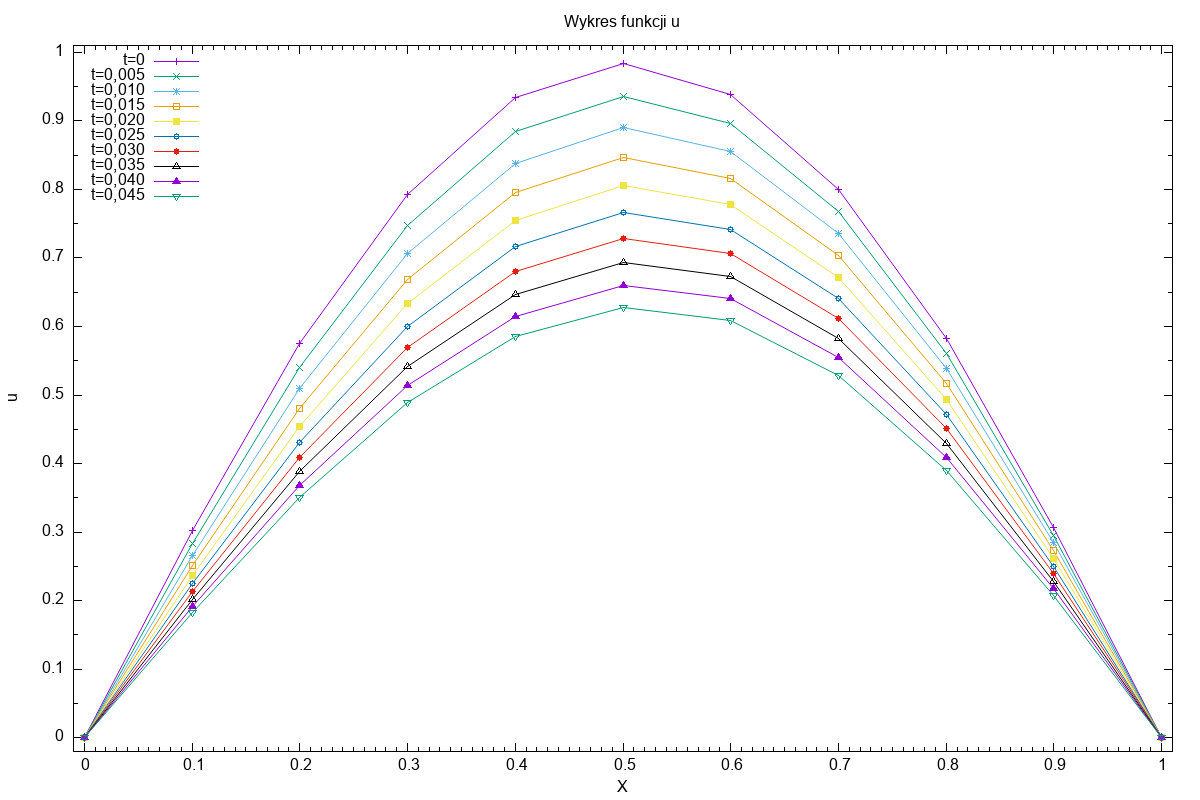
\includegraphics[width=0.7\linewidth]{wykresy dla u(x,t).png}
	\caption{k = 0.005, h = 0.1}
	\label{fig:wykresy-dla-uxt}
\end{figure}
\begin{table}[]
	\begin{tabular}{|l|l|l|l|l|l|l|}
		\hline
x\textbackslash{}t & 0        & 0.005    & 0,010    & 0.015    & 0.020    & 0.025    \\ \hline
0                  & 0        & 0        & 0        & 0        & 0        & 0        \\ \hline
0.1                & 0.301705 & 0.283068 & 0.266381 & 0.251276 & 0.237487 & 0.224811 \\ \hline
0.2                & 0.574577 & 0.540199 & 0.509139 & 0.480833 & 0.454852 & 0.430863 \\ \hline
0.3                & 0.792316 & 0.747317 & 0.706078 & 0.668073 & 0.632879 & 0.600146 \\ \hline
0.4                & 0.933565 & 0.88415  & 0.838007 & 0.794843 & 0.754384 & 0.716382 \\ \hline
0.5                & 0.984036 & 0.93621  & 0.890555 & 0.847073 & 0.805711 & 0.766389 \\ \hline
0.6                & 0.938116 & 0.896627 & 0.856073 & 0.816677 & 0.778584 & 0.741879 \\ \hline
0.7                & 0.799679 & 0.767504 & 0.735313 & 0.703418 & 0.672066 & 0.641447 \\ \hline
0.8                & 0.581939 & 0.560385 & 0.53838  & 0.516199 & 0.494079 & 0.472219 \\ \hline
0.9                & 0.306254 & 0.295543 & 0.284455 & 0.273144 & 0.26175  & 0.250398 \\ \hline
1                  & 0        & 0        & 0        & 0        & 0        & 0        \\ \hline\end{tabular}
	\caption{Wyniki dla k=0.005,h=0.1, dla czasu od 0 do 0.025}
	\label{tab1}
\end{table}
\begin{table}[]
	\begin{tabular}{|l|l|l|l|l|l|}
		\hline
		x\textbackslash{}t & 0.030    & 0.35     & 0.40     & 0.45     & 0.45     \\ \hline
		0                  & 0        & 0        & 0        & 0        & 0        \\ \hline
		0.1                & 0.213091 & 0.202201 & 0.192041 & 0.182528 & 0.182528 \\ \hline
		0.2                & 0.408602 & 0.387857 & 0.368453 & 0.350247 & 0.350247 \\ \hline
		0.3                & 0.569591 & 0.540975 & 0.514101 & 0.488803 & 0.488803 \\ \hline
		0.4                & 0.680618 & 0.6469   & 0.615061 & 0.584955 & 0.584955 \\ \hline
		0.5                & 0.729015 & 0.693493 & 0.659731 & 0.627636 & 0.627636 \\ \hline
		0.6                & 0.706609 & 0.672786 & 0.640407 & 0.609451 & 0.609451 \\ \hline
		0.7                & 0.611699 & 0.582919 & 0.555172 & 0.528496 & 0.528496 \\ \hline
		0.8                & 0.450776 & 0.429873 & 0.409598 & 0.390013 & 0.390013 \\ \hline
		0.9                & 0.239189 & 0.228205 & 0.217507 & 0.207141 & 0.207141 \\ \hline
		1                  & 0        & 0        & 0        & 0        & 0        \\ \hline
	\end{tabular}
		\caption{Wyniki dla k=0.005,h=0.1, dla czasu od 0.030 do 0.045}
	\label{tab2}
\end{table}
Można zauważyć, że jak zmniejszymy k do 0.0005, to można zauważyć, że dla czasu 0 funkcja jest trójkąta. Natomiast dla większego czasu można zauważyć, że funkcja się powoli zaokrągla i~przypomina coraz bardziej wykres dla sinusa, można to zauważyć na rys~\ref{wyk2}. \\
Na pozostały wykresach~\ref{wyk11,wyk12,wyk13}, można zauważyć jak zmiana współczynników wpływa na generowanie wykresów. Jak zmienia się współczynnik lepkości to można zauważyć że amplituda zwiększa się lub zamieszcza, zależy od wartości. Natomiast gdy się zmienia krok przestrzeni to zmienia się ilość punktów na osi~x, a gdy ostatnią wartość się zmieni (krok czasowy), to powstaje więcej lub mniej rozwiązań $\theta$ od czasu.Na każdych z wykresów można zauważyć, że dla coraz większego czasu amplituda zamieszcza się oraz lekko przesuwa się w prawą stronę.\\
Gdy warunek na stabilność, $k/h^2\le0.5$ jest nie zachowany to program wygeneruję wyniki, ale w pliku tekstowym pojawiają się wartości "ind", których nie można przeanalizować oraz naszkicować na wykresie tych punktów. Natomiast gdy zmienia się wartości lepkości, które są niezgodnie dla obliczeń. \\
\begin{figure}[ht]
    \centering
    \subfloat[$\beta$=0.1, k=0.001, h=0.025]{%
        \includegraphics[width=0.3\linewidth]{wykresy dla u(x,t) v=0,1 k = 0.001, h = 0.025.png}
        \label{wyk11}
    }
    \hfill
    \subfloat[$\beta$=0.1, k=0.005, h=0.1]{%
        \includegraphics[width=0.3\linewidth]{wykresy dla u(x,t) v=0,1 k = 0.005, h = 0.1.png}
        \label{wyk12}
    }
    \hfill
    \subfloat[$\beta$=0.99, k=0.005, h=0.1]{%
        \includegraphics[width=0.3\linewidth]{wykresy dla u(x,t) v=0,99 k = 0.005, h = 0.1.png}
        \label{wyk13}
    }
    \caption{Wykresy dla rozwiązań transformaty}
    \label{Wykresy dla rożwiązań}
\end{figure}
Przedstawione na wykresach~\ref{fig:wykresy_dla_rozwiazan}, można zobaczyć, że dla większego czasu, że wykres coraz mniej przypomina wykres sinusa. Może wynikać to z błędach numerycznych, które z każdym rozwiązaniem gromadzą się i robią się coraz większe. Dla $beta=1$ dla trzeba więcej rozwiązań dla czasu niż jest przedstawione dla~\ref{wyk22}, podobnie jest dla wykresu~\ref{wyk21}, jeśli zastosuję się $beta=5$. Ponieważ te wartości są bardzo blisko \begin{equation*}
\beta<\frac{h^2}{2k}
\end{equation*}
\begin{figure}[]
    \centering
    \subfloat[$\beta=10$, $k=0.00001$, $h=0.01$]{%
        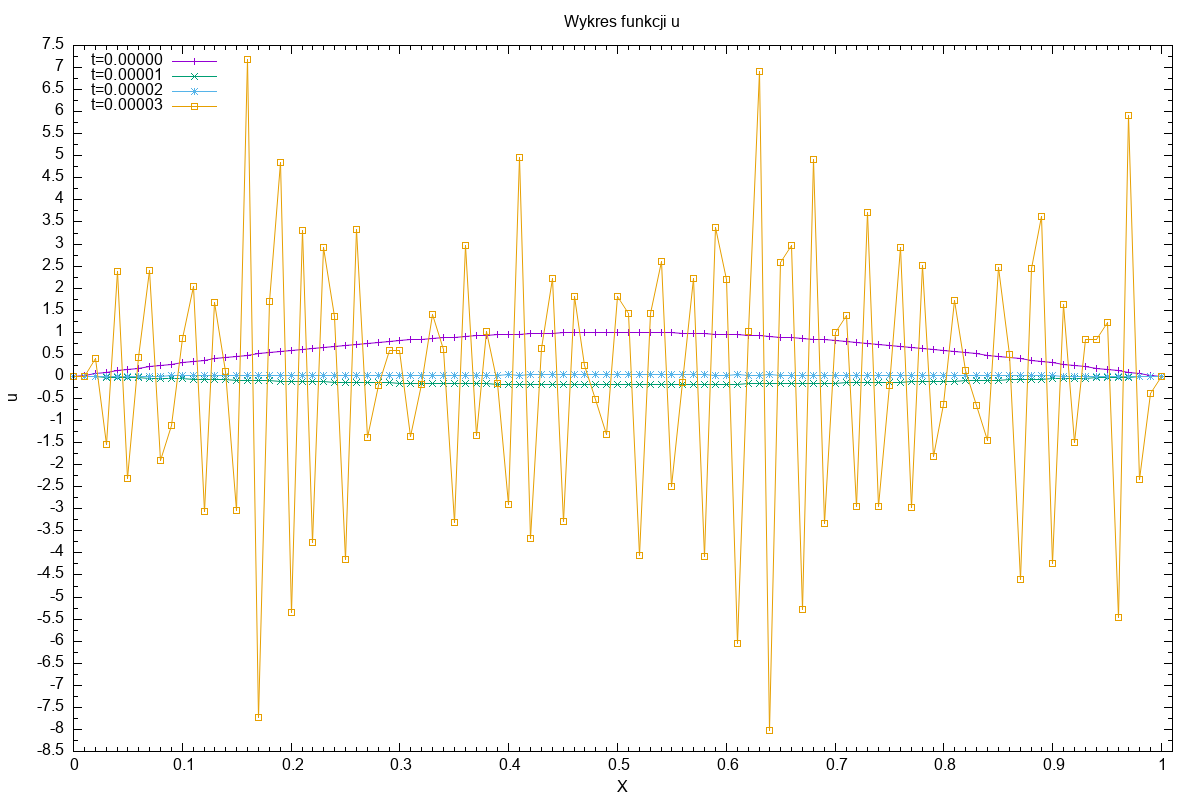
\includegraphics[width=0.45\linewidth]{zl.png}
        \label{wyk21}
    }
    \hfill
    \subfloat[$\beta=5$, $k=0.005$, $h=0.1$]{%
        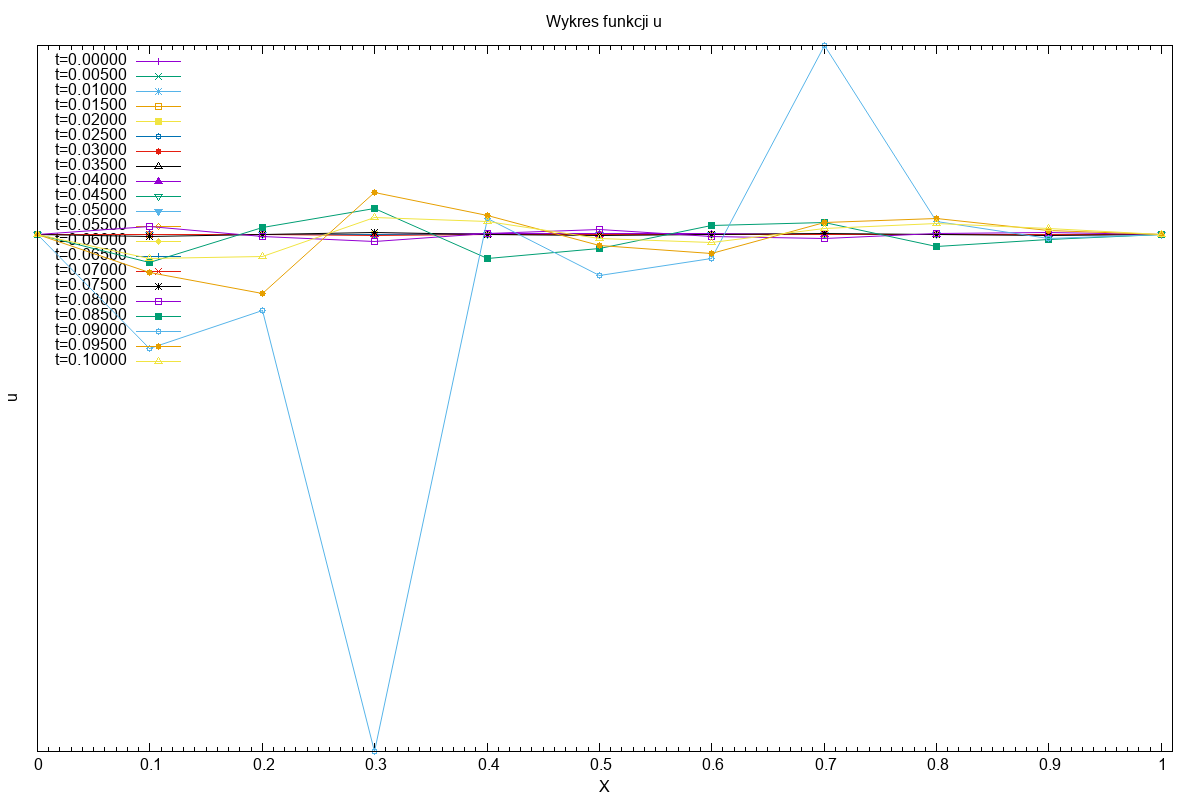
\includegraphics[width=0.45\linewidth]{zl1.png}
        \label{wyk22}
    }
    \caption{Źle dobrane warunki}
    \label{fig:wykresy_dla_rozwiazan}
\end{figure}

\end{document}
